\documentclass[11pt]{article}
\usepackage[margin=1in]{geometry}                % See geometry.pdf to learn the layout options. There are lots.
\geometry{letterpaper}                   % ... or a4paper or a5paper or ... 
%\geometry{landscape}                % Activate for for rotated page geometry
\usepackage[parfill]{parskip}    % Activate to begin paragraphs with an empty line rather than an 
\usepackage{graphicx}
\usepackage{rotating}
\usepackage{amsmath}
\usepackage{amsfonts}
\usepackage{amsthm}
\usepackage{amssymb}
\usepackage{epstopdf}
\usepackage{float}
\usepackage{caption}
\usepackage{url}

\DeclareGraphicsRule{.tif}{png}{.png}{`convert #1 `dirname #1`/`basename #1 .tif`.png}

\title{xJ\"{u}s: Passive-Spine Hexapod \\
Senior Project with Design, Mid-Year Progress Report}

\author{Hayk Martirosyan, Greg Hughes, Thomas Owlett,\\ Brendan O'Leary, and Christopher Payne\\\\
Department of Mechanical and Aerospace Engineering, Princeton University\\
Department of Electrical Engineering, Princeton University
}

%\author{Greg Hughes (MAE '13) 
%\and Chris Payne (ELE '13)
%\and Hayk Martirosyan (MAE '13)
%\and Tom Owlett ('MAE 13)
%\and Brendan O'Leary (MAE '13)}

\date{January 11, 2013}
                                
\begin{document}

\maketitle

\setcounter{section}{-1}
\section{Abstract}

Mid-year progress report of a research and design effort to create a segmented robotic hexapod with a passively compliant spine. The goal of the project is to improve performance of the widely researched RHex design over rough terrain and obstacles by incorporating a flexible backbone to allow for more natural motion, similar to the way that mammals and reptiles conform their bodies during locomotion. A comprehensive simulation was created and a prototype hexapod termed xJ\"{u}s was designed but not yet manufactured. A two-legged test rig was built and achieves successful locomotion. The design of mechanical, electronic, and software systems for the prototype are discussed, as well as preliminary findings from simulation studies and the test rig.

% \tableofcontents

\section{Introduction}

The field of robotics is increasingly utilizing biological mimicry in an effort to capture stable and efficient modes of locomotion seen in nature. In particular, hexapods like cockroaches can traverse a huge range of terrain with relatively little energy. Many hexapodal robots with this biological inspiration have been designed in recent years, but possibly the most successful adaptation is the RHex, spawned from a combination of various research universities, DARPA, and Boston Dynamics\footnote{Boston Dynamics: RHex Rough-Terrain Robot http://www.youtube.com/watch?v=ISznqY3kESI}. By using rotary, compliant legs with a curved shape, the RHex is highly versatile yet at the same time simple enough to require only one active degree of freedom per leg. The RHex and related machines owe their dexterity to various passively actuated compliant degrees of freedom that provide adaptation to the environment at high frequencies and force ranges.\footnote{U. Saranli and M. Buehler and D. E. Koditschek, RHex: A Simple and Highly Mobile Hexapod Robot, http://kodlab.seas.upenn.edu/uploads/Kod/Saranli01.pdf}

\begin{figure}[h]
\centering
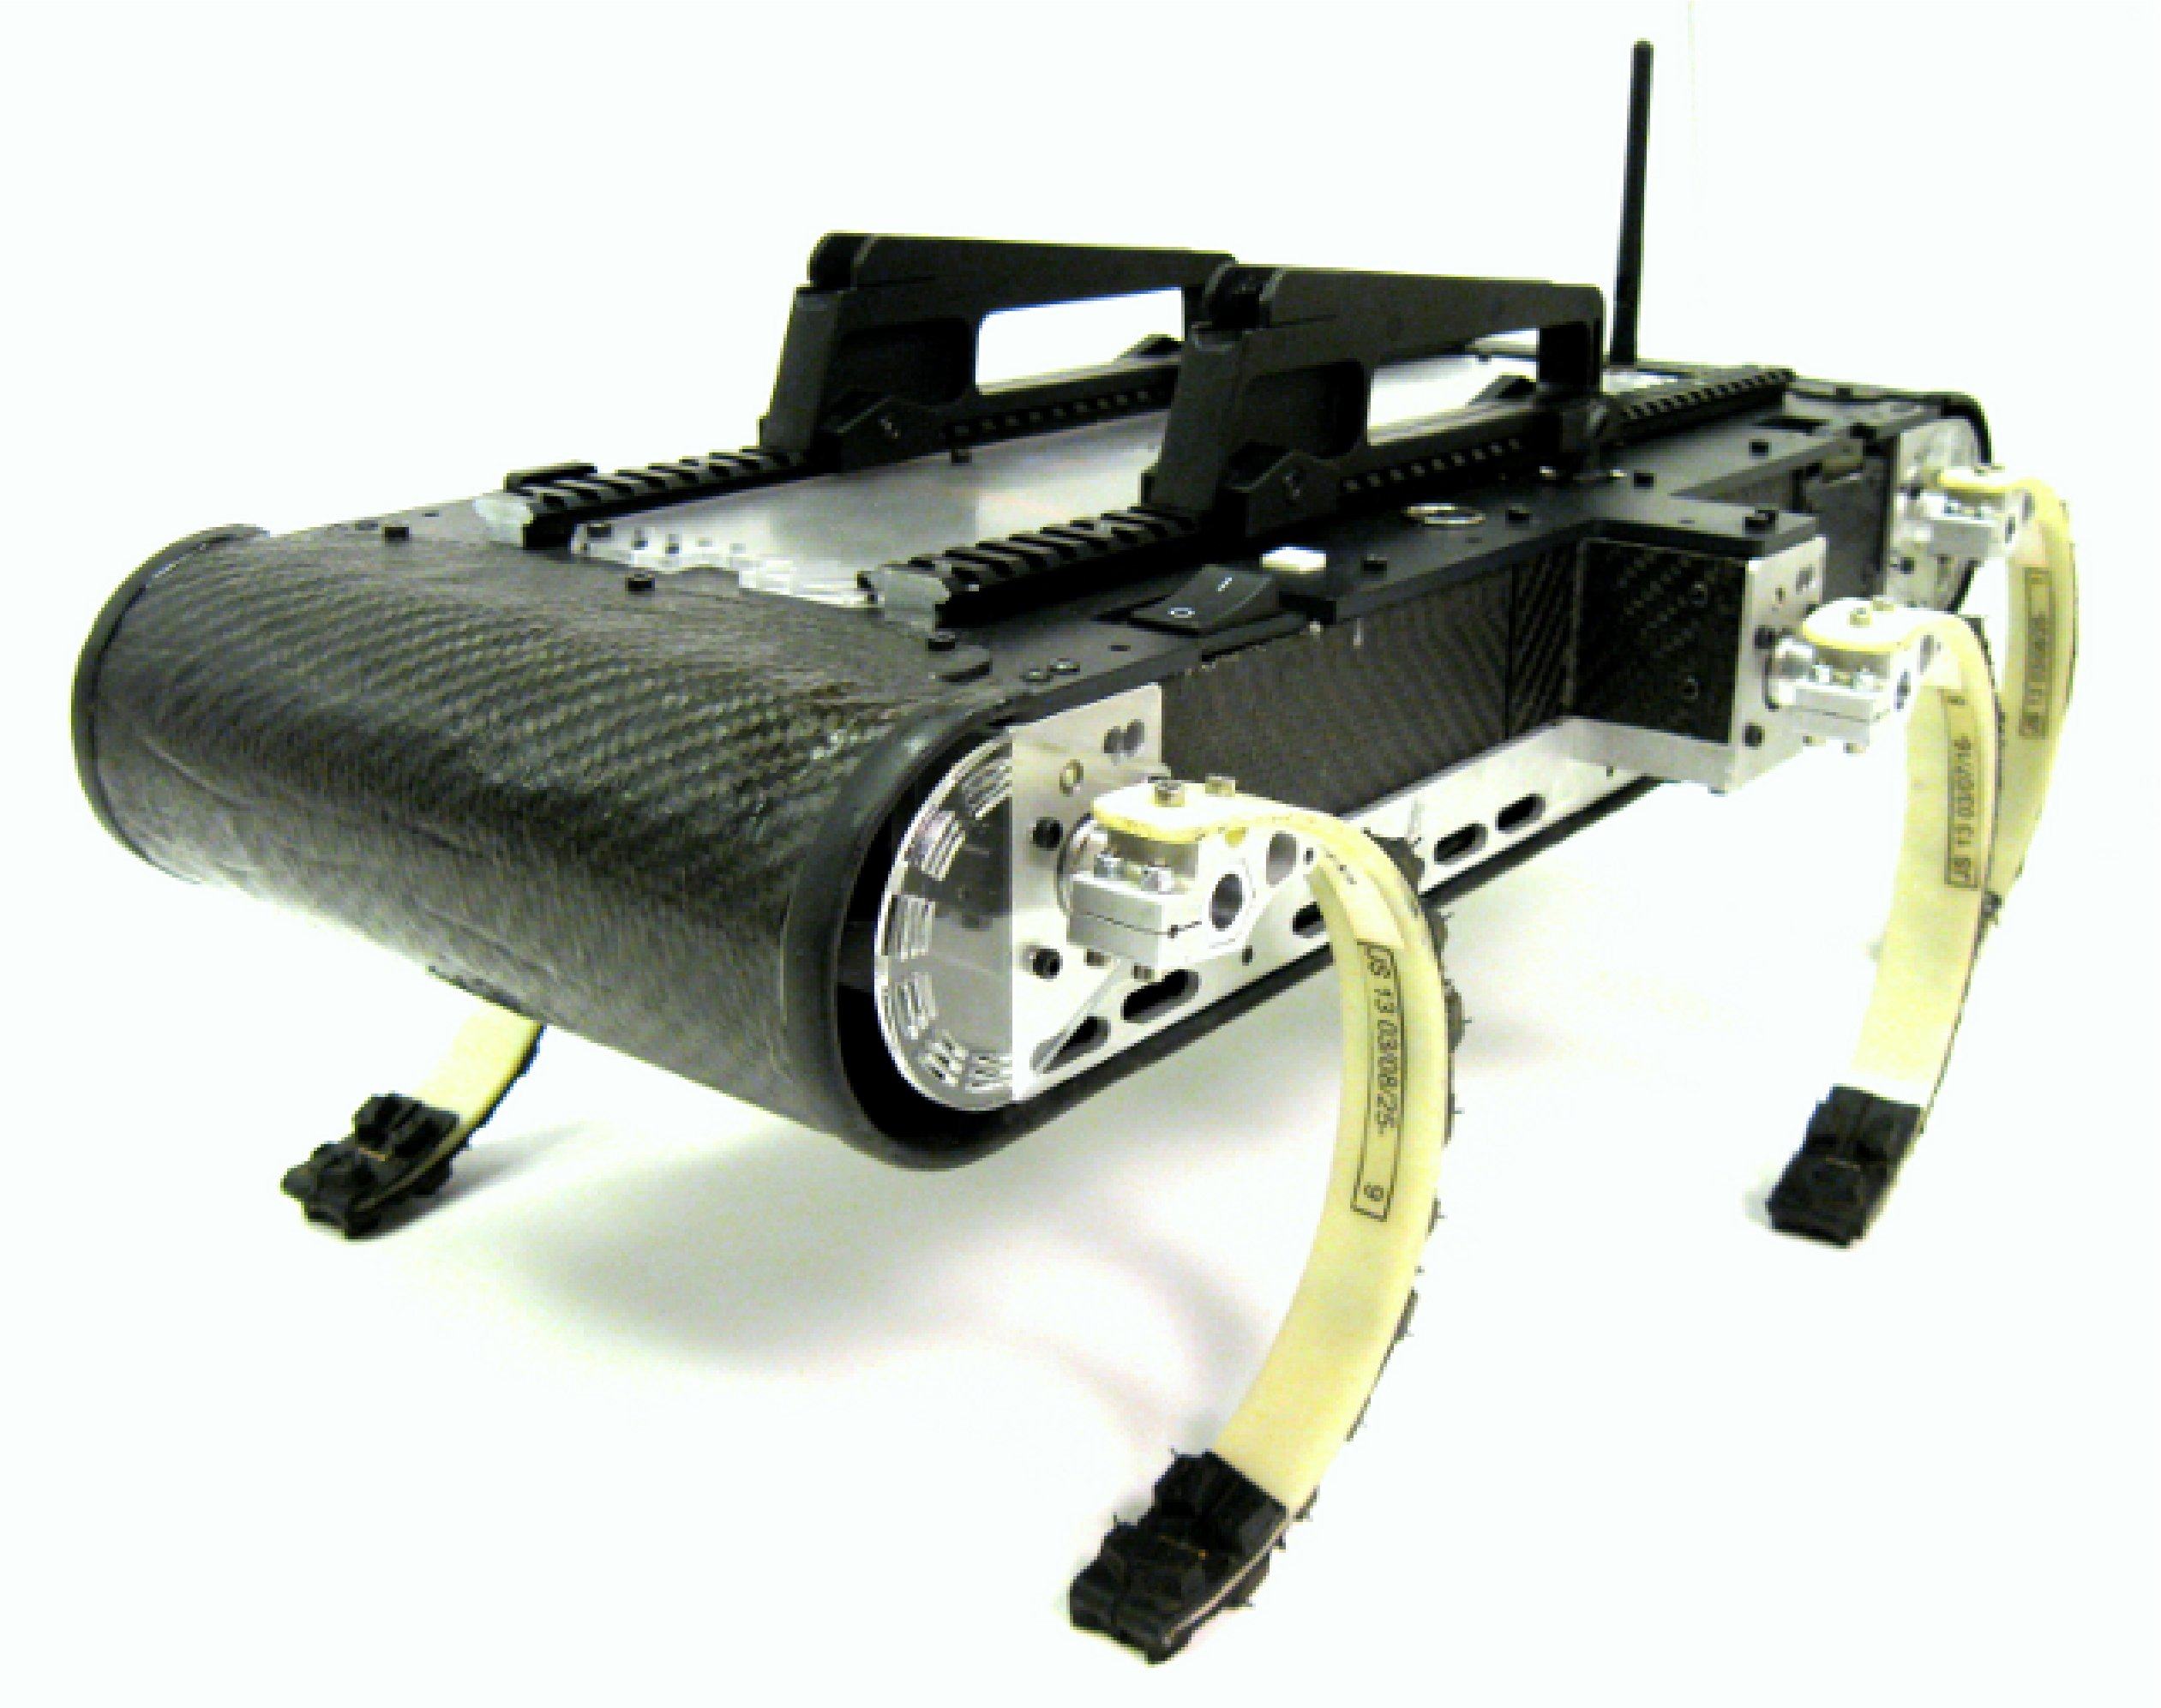
\includegraphics[width=8cm,height=5cm]{RHex.jpg}
\caption{X-RHex, a RHex variant from the University of Pennsylvania}
\end{figure}

This project aims to further model biological locomotion by incorporating a passive backbone into a RHex-like design. Having a fully rigid chassis lacks the flexibility and natural movement of reptiles and mammals, which employ many passive degrees of freedom in their bodies for robust navigation.  Observations from nature and the rigid RHex design suggest that a body with the properly designed passive articulation would lead to improved behavior. Our goal is to design and build a RHex-like hexapod that utilizes this passive backbone to achieve increased stability and energy retention over irregular terrain.

The rigid chassis of the conventional RHex will be divided into three segments, each supporting a single pair of legs and associated electronics. A unique joint has been designed for the purpose of providing two passively actuated degrees of freedom between each of the chassis elements. These segment pairs will be capable of pitching and rolling with respect to each other. The third degree of freedom, yaw, was eliminated due to the instability it introduces in forward locomotion. In total, four degrees of freedom are introduced from the passive spine, in addition to the six active degrees of freedom in the legs. Each of these passive degrees of freedom are independent and have adjustable stiffnesses, with the ability to lock them into place
to act as a rigid chassis.

We are currently at the halfway point for the project and this paper discusses our progress over the past four months. A comprehensive simulation of our design has been built, which allows for open experimentation with the flexible-spine morphology both in terms of physical characteristics and control methods. The hexapod has been fully designed in software and significant analysis has been performed. The bulk of our mechanical and electrical components have been purchased and tested, and a test cart consisting of two legs and two back wheels has been successfully operated.

Moving forward, construction of the final design will commence on schedule. Experiments regarding the performance of our design in terms of stability and efficiency will be performed first on the simulation and later the physical robot. Control methods and high-level locomotion routines will be further developed and fine-tuned. The following sections describe our progress and preliminary findings in detail.

\section{Simulation and Control Methods}

\begin{figure}[ht]
\begin{minipage}[b]{0.45\linewidth}
\centering
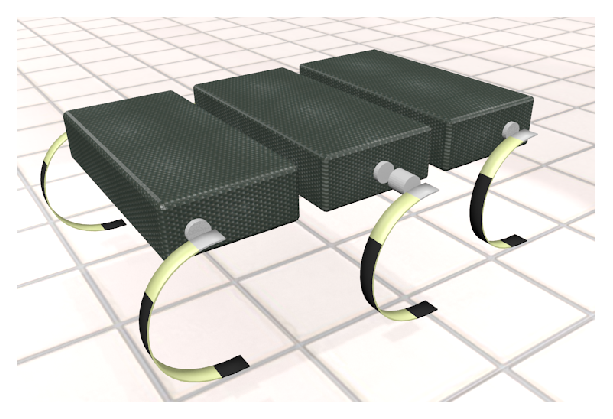
\includegraphics[width=\textwidth]{report_gr1.eps}
\end{minipage}
\hspace{0.5cm}
\begin{minipage}[b]{0.45\linewidth}
\centering
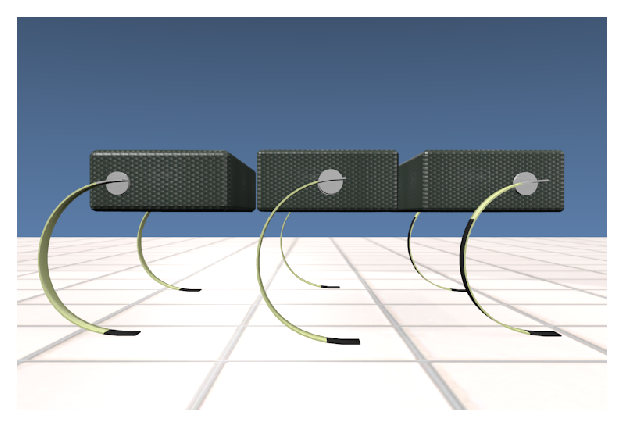
\includegraphics[width=\textwidth]{report_gr2.eps}
\end{minipage}
\caption{Rigid body model in the simulation environment}
\end{figure}

\subsection{Overview}

To motivate our design and create a platform for rapid experimentation, a full and interactive 3D simulation was developed that combines rigid-body physics with custom dynamics and control algorithms. The simulation provides an environment in which the keyboard is used to specify top-level commands such as standing, walking, and turning, which are then interpreted by control algorithms that apply PD feedback to actuate the simulated legs toward desired trajectories. The simulation includes a realistic motor model and consistent units such that various quantitative metrics regarding stability and efficiency can be measured. The result is a real-time interactive tool that can be used to test virtually any modification to the design, optimize parameters, and run experiments over simulated terrains - all with reasonable confidence in the realism of the simulated robot's behavior.
 
\subsection{Simulation Environment}

The simulation was created in Blender\footnote{Blender, http://blender.org}, an open-source 3D graphics program with an embedded version of the Bullet physics engine. Bullet is a very popular engine and is the core physics library used in many well-known games, movies, and simulation environments\footnote{Bullet Physics Library, http://bulletphysics.org}. It includes support for rigid and soft-body dynamics, 6DOF constraints, and accurate friction models. In this simulation, Blender is used to model the 3D bodies that make up the robot and the terrain it traverses, and Bullet is used to handle the rigid-body dynamics between these bodies. The rest of the dynamics, including the motor models and compliant spine joints, are programmed in Python and interact with Bullet by applying forces and torques to the rigid bodies. Blender is written entirely in Python\footnote{Blender Python API, \url{http://www.blender.org/documentation/blender_python_api_2_65_5/}} and the simulation was made using a combination of the graphical interface and written Python code. OpenGL is used for real-time rendering at 120FPS with five physics substeps per frame, resulting in a working simulation timestep of 1.7 milliseconds and a logic timestep of 8.3 milliseconds. Arbitrarily small timesteps are achievable if recorded data instead of real-time interactivity is sufficient.

The robot model is a simplified version of the planned final design, consisting of rigid body segments constrained to each other with specified degrees of freedom. Each body has an associated mass, inertia tensor, and collision mesh. Three identical chassis segments each have box collision meshes, and are attached together to allow pitching and rolling but not yawing, as can be seen in Figure \ref{fig:simulationwalking}. Each leg system consists of one motor cylinder fixed to the chassis and one motor cylinder fixed to the leg. Each pair of motor cylinders are allowed relative rotation about their shaft axis, providing one degree of freedom per leg. The legs are modeled as thin curved strips, but their collision meshes are treated as convex due to significant performance gains. 

\begin{figure}[t]
\begin{minipage}[b]{0.45\linewidth}
\centering
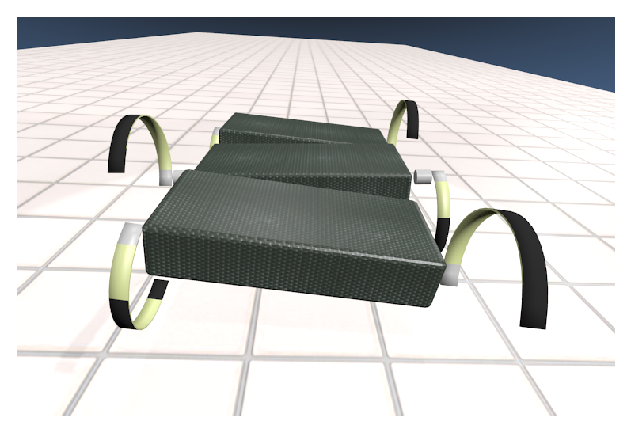
\includegraphics[width=\textwidth]{report_gr4.eps}
\end{minipage}
\hspace{0.5cm}
\begin{minipage}[b]{0.45\linewidth}
\centering
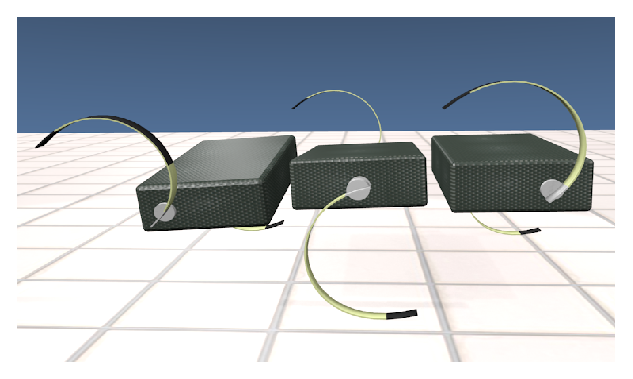
\includegraphics[width=\textwidth]{report_gr5.eps}
\end{minipage}
\caption{Simulated walking routine with compliant chassis segments}
\label{fig:simulationwalking}
\end{figure}

Every polygon is assigned a material that has associated coefficients of friction and elasticity (restitution), as well as properties of its appearance within the simulation. Each texture in the simulation corresponds to a different material with realistic coefficients chosen to mimic what our final design would have. For every collision between two polygons, the physics engine takes into account the fricton and elasticity coefficients of both colliding materials.

Efforts were made to ensure the quantitative rigor of this platform. A simple pendulum constructed in Blender yielded identical periods and trajectories to numerical solutions in \textit{Mathematica}\footnote{Wolfram Mathematica, http://www.wolfram.com/mathematica/} for varying masses and lengths. The results remained consistent when damping and forcing was applied using Python, in an identical manner to actuation applied in the robot simulation. All signs show that mass, length, and time units in the simulation are consistent with expectations and measurements can be considered fairly rigorous. Blender is a growing platform for robotics with developing support\footnote{Blender for Robotics, http://wiki.blender.org/index.php/Community:Science/Robotics}, and multiple robotics frameworks have been created based on the combination of Blender and Bullet, the most prolific of which
is MORSE\footnote{MORSE, http://www.openrobots.org/morse/doc/stable/morse.html}, a platform used by several research laboratories. Though this project did not use one of these established frameworks, the core methods
remain identical.

\subsection{Motor Model}

Actuation of the six legs is simulated by a motor model and set of control algorithms primarily based on previous literature regarding the RHex platform.
The motor model computes the output torque $\tau $ for a given leg based on the input voltage \(V_{\text{pd}}\), the shaft angular velocity \(\dot{\theta
}\), and various motor-specific parameters. The model used is taken from previous work\footnote{Justin Seipel, Pei-Chun Lin and Philip Holmes. "RHex-SLIP: A Model of the Robotic Hexapod RHex in the Sagittal Plane. 2006}, where the output torque $\tau $ is given by:

\begin{center}
\(\tau =\eta  N K_t \left(\frac{d V_s-K_s\dot{\theta }}{R_a+d^2R_{\text{amp}}}\right)\)
\end{center}

where d is the dimensionless duty factor that relates the applied voltage \(V_{\text{pd}}\) to the source voltage \(V_s\):

\begin{center}
\(d=\max \left\{-1, \min \left\{+1, \frac{V_{\text{pd}}}{V_s}\right\}\right\}\)
\end{center}

The system parameters are given in Table~\ref{table:parameters}. They are taken from the specifications of purchased components, except for \(K_t\) and \(K_s\), which were chosen such that the model reflects the stall torque and no load speed of the motor.

\begin{center}
\(\begin{array}{ccc}
 \textbf{Symbol} & \textbf{Constant} & \textbf{Value} \\
 N & \text{gear ratio} & \frac{729}{25} \\
 \eta  & \text{net efficiency} & 0.60 \\
 V_s & \text{source voltage} & 22.2V \\
 R_a & \text{motor resistance} & 2.36\frac{V}{A} \\
 R_{\text{amp}} & \text{amplifier resistance} & 0.5\frac{V}{A} \\
 K_t & \text{conversion factor} & 0.016\frac{N m}{A} \\
 K_s & \text{conversion factor} & 0.75V s \\
\end{array}\)
\captionof{table}{System Parameters}
\label{table:parameters}
\end{center}

This model represents a linear torque-speed curve. Curves for various duty cycles are shown by Figure \ref{fig:dutycyclecurves}.

\begin{figure}[H]
\centering
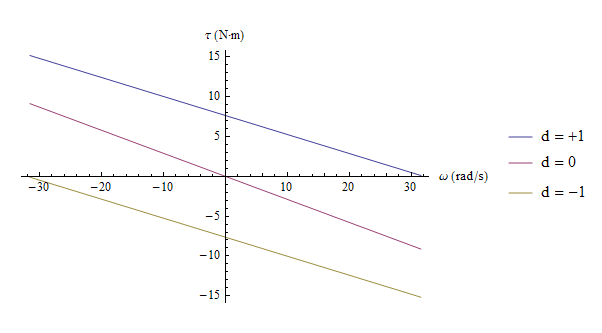
\includegraphics{report_gr6.eps}
\caption{Duty Cycle Curves}
\label{fig:dutycyclecurves}
\end{figure}

\subsection{Control System}

The simulation uses a modular hierarchy of control methods that serve to translate high-level commands received from the keyboard into torques applied to the motor-cylinder rigid bodies. The very last step of actuation is to provide a feedback voltage \(V_{\text{pd}}\) to the motor model, which then outputs a torque $\tau$ and reaction torque -$\tau$ to the relevant pair of motor cylinders using the equations described in the previous section.

Calculating \(V_{\text{pd}}\) for each leg first requires generating a target trajectory for each leg. When the user invokes a keyboard command, a locomotion routine is activated which signifies a high-level motion such as walking, turning, or standing in place. For each leg, the high-level routine calls a trajectory generation function that calculates a desired angle function \(\theta _d(t)\). The trajectory generation function is called with various parameters such as the desired period of revolution, ground contact angle, turning magnitude, and relative timings of the legs, dependent on the goals of the chosen high-level routine. \(\theta _d(t)\) outputs the target angle of a certain leg at any time t measured from start of the routine. The method of calculating \(\theta _d(t)\) is discussed in the following section for clarity.

Once leg target angles are calculated for a given simulation frame, the high-level routine invokes a simple proportional-derivative feedback loop to calculate the motor input \(V_{\text{pd}}\). The feedback loop takes the following error \(\theta -\theta _d\) and uses specified gains \(k_p\) and \(k_d\) to calculate \(V_{\text{pd}}\), which is fed to the motor model for low-level actuation.

Assuming a simple motor plant:

\begin{center}
\(\tau =J \overset{\cdot \cdot }{\theta }\)
\end{center}

A basic LTI state space for the shaft angle $\theta $ of a leg is given by:

\begin{center}
\(\frac{d}{dt}\left(
\begin{array}{c}
 \theta  \\
 \dot{\theta } \\
\end{array}
\right)=\left(
\begin{array}{cc}
 0 & 1 \\
 0 & 0 \\
\end{array}
\right)\left(
\begin{array}{c}
 \theta  \\
 \dot{\theta } \\
\end{array}
\right)+\left(
\begin{array}{c}
 0 \\
 \frac{1}{J} \\
\end{array}
\right)\tau\)
\end{center}

Changing variables from the angle $\theta $ to the angle error \(\theta -\theta _d\):

\begin{center}
\(x=\left(
\begin{array}{c}
 \theta -\theta _d \\
 \dot{\theta }-\dot{\theta _d} \\
\end{array}
\right)\)

\(\dot{x}=\left(
\begin{array}{cc}
 0 & 1 \\
 0 & 0 \\
\end{array}
\right)x+\left(
\begin{array}{c}
 0 \\
 1 \\
\end{array}
\right)\overset{\cdot \cdot }{\theta _d}-\left(
\begin{array}{c}
 0 \\
 \frac{1}{J} \\
\end{array}
\right)\tau\)
\end{center}

\(\overset{\cdot \cdot }{\theta _d}\) is a feedforward term that represents the acceleration of the generated trajectory, a known function. By substituting
\(u\) as a generic input, we simplify:

\begin{center}
\(u=\overset{\cdot \cdot }{\theta _d}-\tau /J\)

\(\dot{x}=\left(
\begin{array}{cc}
 0 & 1 \\
 0 & 0 \\
\end{array}
\right)x+\left(
\begin{array}{c}
 0 \\
 1 \\
\end{array}
\right)u\)
\end{center}

Applying state feedback for PD control, an expression for the desired torque output $\tau $ is derived:

\begin{center}
\(u=-K x=-\left(
\begin{array}{cc}
 k_p & \left.k_d\right)x \\
\end{array}
\right.\)

\(\tau /J-\overset{\cdot \cdot }{\theta _d}=\left(
\begin{array}{cc}
 k_p & \left.k_d\right)x \\
\end{array}
\right.\)

\(\tau =J\left(\overset{\cdot \cdot }{\theta _d}+
\begin{array}{cc}
 \left(k_p\right. & \left.\left.k_d\right)\left(
\begin{array}{c}
 \theta -\theta _d \\
 \dot{\theta }-\dot{\theta _d} \\
\end{array}
\right)\right) \\
\end{array}
\right.\)

\(\tau =J\left(\overset{\cdot \cdot }{\theta _d}+k_p\left(\theta -\theta _d\right)+k_d\left(\dot{\theta }-\dot{\theta _d}\right)\right)\)
\end{center}

This is the control algorithm for $\tau $. Combined with the motor model, this is a formal method of calculating \(V_{\text{pd}}\) for every frame,
assuming the trajectory function is known. The following section discusses how \(\theta _d(t)\) is calculated.

\subsection{Trajectory Generation}

The primary trajectory generation function expands on the fundamental tripod gait of the RHex morphology\footnote{U. Saranli, M. Buehler, and D.E. Koditschek. RHex: A simple and highly mobile hexapod robot. Int. J. Robotics Research, 20(7):616-631, 
2001}. The main idea for this walking trajectory is that three legs are contacting the ground at all times, providing a stable base for locomotion. Given a revolution period T, each leg spends half the period sweeping a ground contact angle \(\theta _g\) (generally 45${}^{\circ}$-90${}^{\circ}$) slowly, and then comes full circle over the air angle \(\theta _a\) with the second half of the revolution period. The velocity of this profile is a periodic piecewise constant function given by:

\begin{center}
\(\dot{\theta _d}(t)=\left\{
\begin{array}{cc}
 \omega _g & 0\leq mod(t, T) <\frac{T}{2} \\
 \omega _a & \frac{T}{2}\leq mod(t, T) <T \\
\end{array}
\right.\)
\end{center}

where \(\omega _g\) and \(\omega _a\) are the ground and air velocities, derived from \(\theta _g\) and T:

\begin{center}
\(\theta _a=360{}^{\circ}-\theta _g\)\\
\(\omega _g=2\frac{\theta _g}{T}\)\\
\(\omega _a=2\frac{\theta _a}{T}\)
\end{center}

To avoid the use of piecewise functions and to smooth the ground contact transition, a Fourier series of \(\dot{\theta _d}(t)\) is used instead of
the original. This has the benefit of being a continuous function that is easier to deal with both programatically and mathematically. The Fourier series of \(\dot{\theta _d}(t)\) with M nonzero terms when fully simplified is given by:

\begin{center}
\(\dot{\theta _d}(t)=\frac{2 \pi }{T}+\sum _{m=1}^M \frac{8\left(\theta _g-\pi \right)}{(2m-1)\pi  T}\sin \left(\frac{2\pi  (2m-1)}{T}t\right)\)
\end{center}

\begin{figure}[H]
\centering
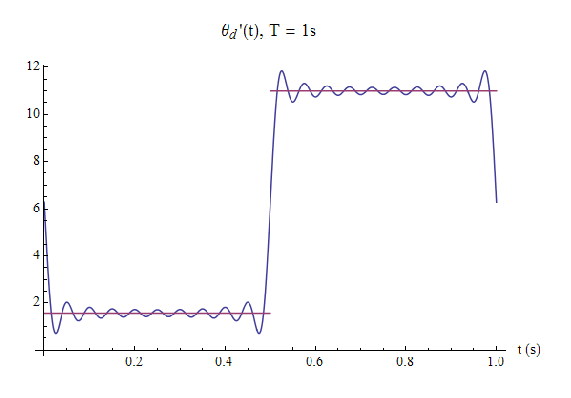
\includegraphics{report_gr7.eps}
\caption{A plot of \(\dot{\theta _d}(t)\) for \(T=1s\), \(\theta _g=45{}^{\circ}\), and M = 10, with both the piecewise and Fourier variants.}
\label{fig:piecewise}
\end{figure}

The Fourier approximation of \(\dot{\theta _d}(t)\) is easily differientiable to yield an expression for \(\theta _d(t)\):

\begin{center}
\(\theta _d(t)=\left(\frac{2 \pi }{T}\right)t+\sum _{m=1}^M \frac{4\left(\theta _g-\pi \right)}{(2m-1)^2\pi ^2}\left(1-\cos \left(\frac{2\pi  (2m-1)}{T}t\right)\right)\)
\end{center}

Figure \ref{fig:angleposition} shows \(\theta _d(t)\) for the same trajectory as the plotted \(\dot{\theta _d}(t)\), and we see the result is highly linear, but with a smooth transition between the ground and air regimes.

\begin{figure}[H]
\centering
\includegraphics{report_gr8.eps}
\caption{Fourier approximation of \(\theta _d(t)\),} the shaft angle, for one revolution
\label{fig:angleposition}
\end{figure}

It is this function that is used by the the trajectory generation function of the simulation, and will also be used for control the physical robot. By varying \(\theta _g\), T, and the starting time of each leg's trajectory, a wide range of locomotion routines are achieved. This method of trajectory generation has been successfully demonstrated for the simulation as well as for driving our actual motors.

\subsection{Next Steps}

At the current stage of development, the simulation is an accurate representation of the dynamics of our proposed flexible-spine hexapod. Moving forward, it will be used as a testbed for optimizing parameters and general experimentation to guide our design decisions as plans for construction of the physical robot prototype are finalized. Formal simulated experiments comparing the compliant chassis joints to a fully rigid chassis have not yet been conducted, but qualitative results show some improved behavior over rough terrain. Simulated experiments will be conducted using various metrics of stability and efficiency to further motivate our novel step and build reasonable expectations for our final design. For example, power usage over stochastically generated terrain can be measured for various joint stiffnesses. Once construction is complete, analogous experiments will be attempted with the final design and results will be compared for further evaluation of the simulation platform.

\begin{figure}[H]
\centering
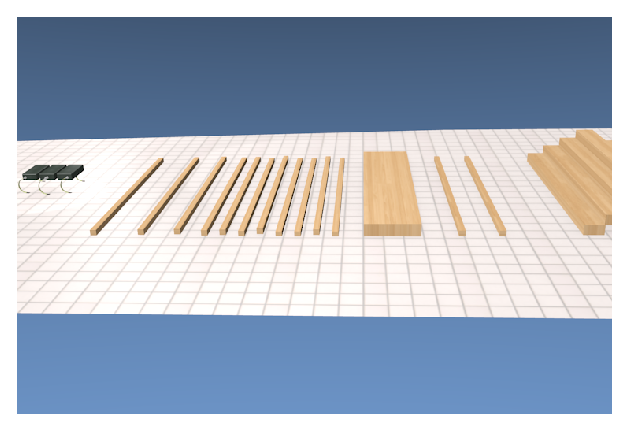
\includegraphics[width=12cm,height=7cm]{report_gr3.eps}
\caption{Example of a simulated obstacle course}
\end{figure}

\section{Design}

\begin{figure}[ht]
\begin{minipage}[b]{0.45\linewidth}
\centering
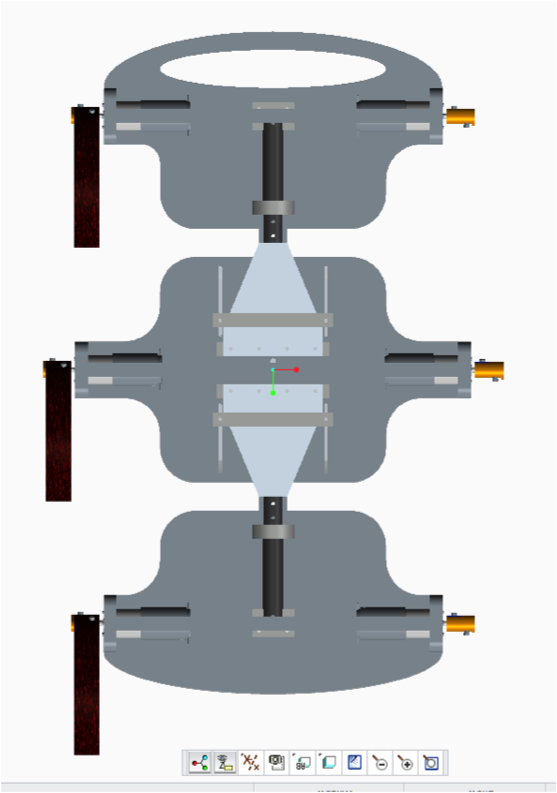
\includegraphics[width=6.5cm, height=9cm]{Xjus2.png}
\end{minipage}
\hspace{0.5cm}
\begin{minipage}[b]{0.45\linewidth}
\centering
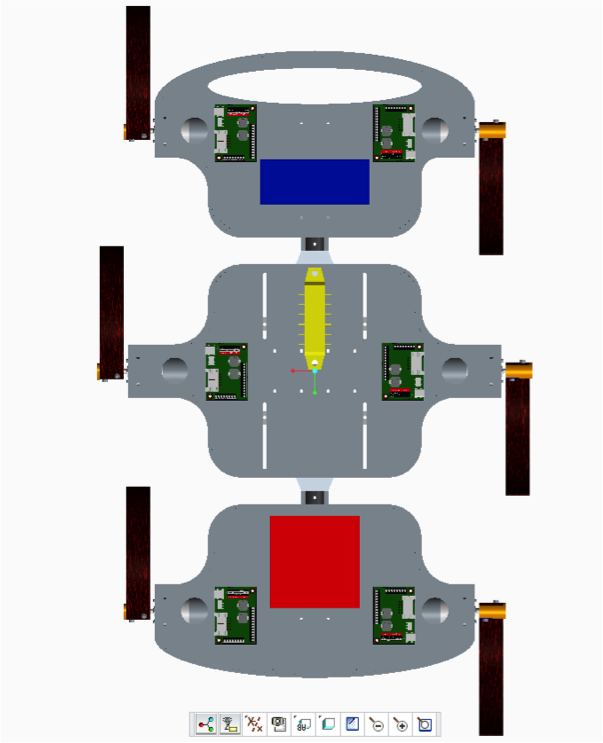
\includegraphics[width=7.5cm,height=9cm]{Xjus3.png}
\end{minipage}
\caption{Planar views of our design. Left: Bottom View. Right: Top View.}
\end{figure}

\subsection{Overview}

Our objective is to design and build a hexapod that expands upon previous RHex variants\footnote{RHex variants, \url{http://www.rhex.web.tr/}} by incorporating a passive backbone that increases versatility and stability. Constructing this robot is a considerable undertaking given our time constraints, so a large focus is put on simplicity of design and modularity. The core of our research effort is dedicated to the design and implementation of a passive backbone allowing two degrees of freedom between the chassis segments. For this reason, we have adapted a similar morphology for the body and legs as that used in the Research RHex\footnote{Research RHex, \url{http://kodlab.seas.upenn.edu/RHex/ResearchRHex}} and Edubot\footnote{EduBot, \url{http://kodlab.seas.upenn.edu/RHex/EduBot}}. Many of our mechanical and electrical systems are modeled after those of the Edubot, but on a larger scale, similar to that of the Research RHex.

The primary focus of mechanical design was placed on the joints between chassis segments. After considering the use of torsion springs for the compliant degrees of freedom in each joint, we opted for an alternative mechanism using tapered beams of spring steel. An adjustable fulcrum along the median of the tapered beam controls the pitch and the placement of a clamp along the length of a rectangular beam adjusts the amount of roll. With the design of the joint complete, our plan is to build a model of the joint to confirm its motion capabilities before we manufacture the rest of the hexapod. The dimensions of body components are currently similar to the Research RHex, but further simulation studies will be done to optimize parameters. Additionally, we opted to use spring steel for the compliant legs rather than composites to simplify manufacturing.

Our electrical system was designed with simplicity in mind, taking advantage of off-the-shelf components whenever possible. Each motor stack consists of a 22-Watt DC motor with a 33:1 planetary gearbox, an encoder, and a Maxon EPOS2 digital position controller. The motor controllers are connected in a CAN network and receive commands from an onboard Linux CPU. Considerable time has been and will continue to be attributed to interfacing with the motor controllers to achieve desired motor performance. Primary power is supplied by a 2200mAh 22.2v LiPo battery, and the CPU will have an auxiliary battery.

Based off of the electrical components already purchased and the current dimensioning of the mechanical components in our design, the robot's estimated weight is 4467g or 9.85lbs. This is significantly lighter than the Research RHex, totaling 8200g. The higher power to weight ratio of our robot will enable more gait patterns and locomotion strategies.

Our initial budget estimate for this project was \$5725 for all mechanical and electrical parts. So far a total of \$4574.88 has been spent, \$269.45 of which was added to our initial estimate, such as a battery charger and supplies for the manufacture of the test cart. 

\begin{figure}[H]
\centering
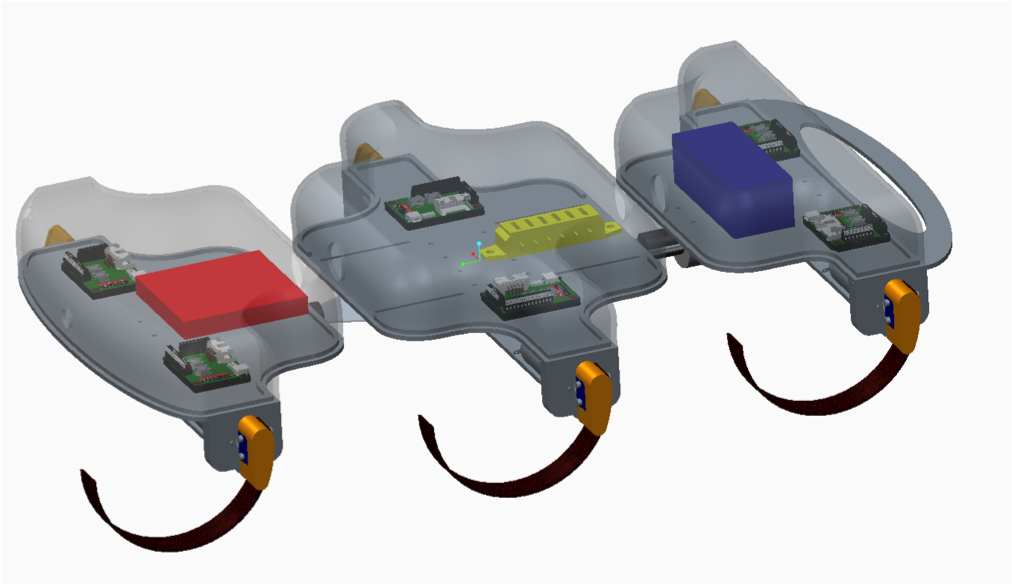
\includegraphics[width=14cm,height=7cm]{Xjus1.png}
\caption{CAD model, 3D view}
\end{figure}

\subsection{Actuation and Power System}

Given the estimated parameters of our design, we can estimate the torque needed for locomotion via the tripod gait:

\begin{figure}[H]
\centering
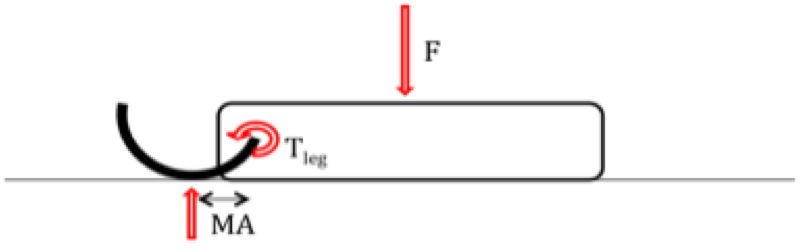
\includegraphics[width=10cm,height=3cm]{torquecalc.png}
\caption{Free body diagram for motor torque calculation}
\end{figure}

\begin{center}
Moment Arm $MA = 1.5"$ \\
Force $F =  M = 10lbf$ \\
Torque applied by motors $T_{tot} = F*MA = 15lbf{\cdot}in$ \\
Torque per leg $T_{leg} = T_{tot}/3 = 5 lbf{\cdot}in = \bf{0.565Nm}$
\end{center}

\vspace{0.25cm}

This is the maximum moment arm applicable to the tripod gait, in the case of effectively lifting the chassis from the ground with only three legs. Typical locomotion will require less torque, and standing up from a rest position will utilize all six legs.

Using the upper bound of the torque needed per leg of 0.565 Nm, this value can be scaled to an associated current draw upper bound. Using the motor torque conversion factor of 25.8 mNm/A and keeping in mind the gearbox ratio of 729/25 we arrive at a maximum current load of 0.75A, which is approximately 25\% below the maximum continuous current rating of 1.08A per motor.

\begin{center}
$ 565 mNm * (25.8 mNm/A)^{-1} * (729/25) ^{-1}= 0.75 A $
\end{center}

We selected a Blue LiPo battery with a capacity of 2.2Ah to service the motors, providing a lower bound of 29 minutes of runtime.

\begin{center}
$ (0.75 A/\text{leg}) * (6\text{ legs}) *(2.2Ah)^{-1} = \text{29 min} $
\end{center}

In reality runtime will be much longer as this calculation assumes a maximum torque load. As we continue to develop the power system and software simulations we will have a have a better picture of the true torque profile and its accompanying power use, a relationship dictated by  both the motor torque conversion power and inefficiencies in the motor controller, motor and accompanying wires.  The chosen battery carries a voltage of 22.2V as a result of 6 internal 3.7V LiPo cells, a voltage that is related to the motor characteristics through the following relation:

\begin{center}
  \item \(V_{\text{s}}=1(V)+\frac{U_N}{n_0}\cdot \left(\frac{\text{$\Delta $n}}{\text{$\Delta $M}}\cdot M_B+n_B\right)\cdot \frac{1}{0.9}\)
\end{center}

\emph{Known values:}

\begin{itemize}
  \item Operating torque \(M_B [\text{mNm}]\)
  \item Operating speed \(n_B \left[\min ^{-1}\right]\)
  \item Nominal motor voltage \(U_N [\text{Volt}]\)
  \item Motor no-load speed at \(U_N, n_0 \left[\min ^{-1}\right]\)
  \item Speed/torque gradient of the motor $\Delta $n/$\Delta $M \(\left[\min ^{-1} \text{mNm}^{-1}\right]\)
\end{itemize}

These voltage and run-time characteristics matched our electrical needs and most importantly provided the power in a high density form to minimize the weight of the hexapod. Table ~\ref{table:battery} compares the vital characteristics of our design's battery to that of the EduBot. For added protection, all individual power lines leading from the battery bus to the motors will be fused at 2A. A bypass capacitor might be tied to the battery output to dampen high frequency voltage fluctuations that affect the controller operation. The BeagleBoard-XM will be operated on a separate 5VDC power source to isolate the digital electronics from the voltage fluctuations caused by the inductive nature of the motors. Currently we are powering the board using a desktop mounted 5VDC power source but will be moving to a mobile battery pack after a suitable one has been selected.

\begin{table}[ht]
\centering
\begin{tabular}{ccc}
\hline
\textbf{Attribute} & \textbf{xJ\"{u}s} & \textbf{EduBot} \\
\hline
Battery Type & LiPo & Lipo \\
Bus Voltage [V] & 22.2 & 14.8 \\
Battery Capacity [Wh] & 48.8 & 20-30 \\
Battery Quantity & 1 & 1-2 \\
Dimensions [mm] & 35 x 104 x 43 & 66 x 74 x 34-50 \\
Battery Mass [g] & 401 & 122-160 \\
Robot Mass Dedicated to Battery [\%] & 8.9 & 3.6-8.9 \\
Battery Energy Density [Wh/kg] & 122 & 158-187 \\
Robot Energy Density [Wh/kg] & 10.8 & 5.8-16.7 \\
\hline
\end{tabular}
\captionof{table}{Comparison of battery properties}
\label{table:battery}
\end{table}

We can also estimate the power draw of our motors, approximated with the target motor torque operating at 3rps:
 \begin{center}
$P_{leg} = T*w = 0.5Nm*3(2\pi) = 9.42 W$ (per leg) \\
$P_{tot} = 6(9.42W) = 56.5W$
\end{center}

This is a rough estimate of the maximum continuous power output needed for the tripod gait. This value must be divided by the efficiencies of the motor, gearbox, and controller to calculate the power draw needed from the battery.

\subsection{Structural Components}

The chassis segments consist of three 0.25" aluminum plates connected by two compliant joints. Each section has its own carbon fiber housing above it to protect the electronics from damage and dirt.  The aluminum plates have cutout recesses to reduce the robot's weight without compromising the structural integrity.  Because the joint allows for roll and pitch between the plates, there is much less torsional stress between the body segments as the robot switches from one set of legs to the other.  To minimize chassis weight, sensitivity studies will be conducted to optimize the removal of material from the cutout sections.

The legs of the robot are constructed using 1074/1075 spring steel.  This steel was chosen for its ability to deform elastically and recover some spent mechanical energy, as well as its relatively high yield strength (50,000 psi).  The formula used to determine the dynamic force for the finite element analysis is:

\begin{center}
$ \text{Dynamic Load} = \frac{\text{Robot Mass}}{\text{\# of Contact Legs}}*\text{Dynamic Load Factor}*g $
\end{center}

A dynamic load factor of 2 was selected for the legs for consistency with the flexible joint deformation calculations.  Using the estimated total robot mass of 4.467 Kg, the dynamic load for each leg is 29.2 N.  Figure \ref{fig:legstress} shows the simulated displacement and stress using this calculated dynamic load and a spring steel thickness of 0.072 inches.  The simulation shows a maximum displacement of 0.30 inches and a maximum stress of 22,888 psi, which is well below the yield stress of 50,000 psi.

\begin{figure}[h]
\centering
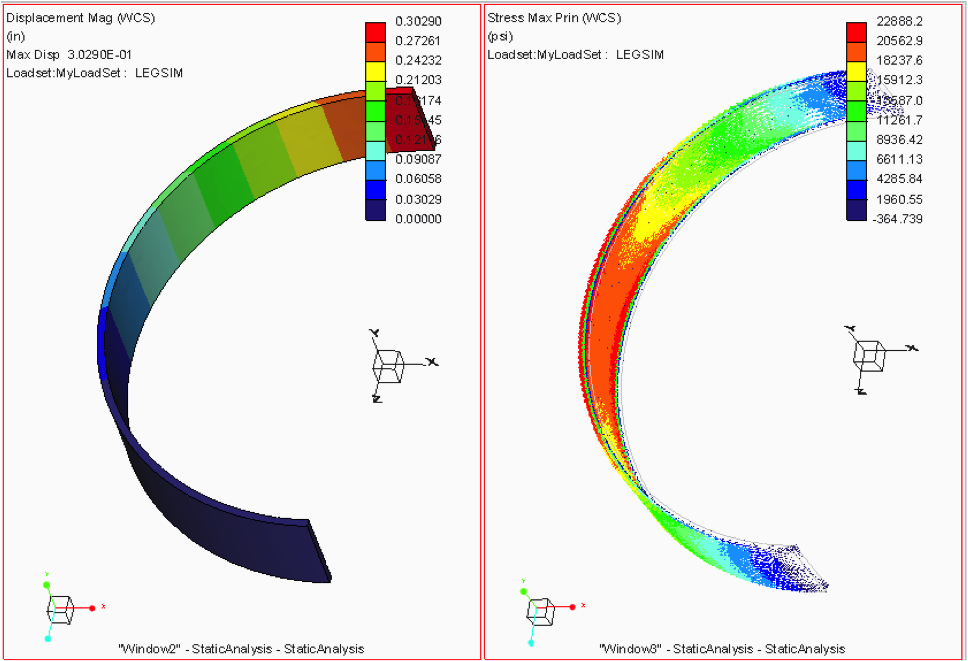
\includegraphics[width=10cm,height=7cm]{leg_analysis.png}
\caption{Leg stress and displacement under load}
\label{fig:legstress}
\end{figure}

\begin{figure}[ht]
\centering
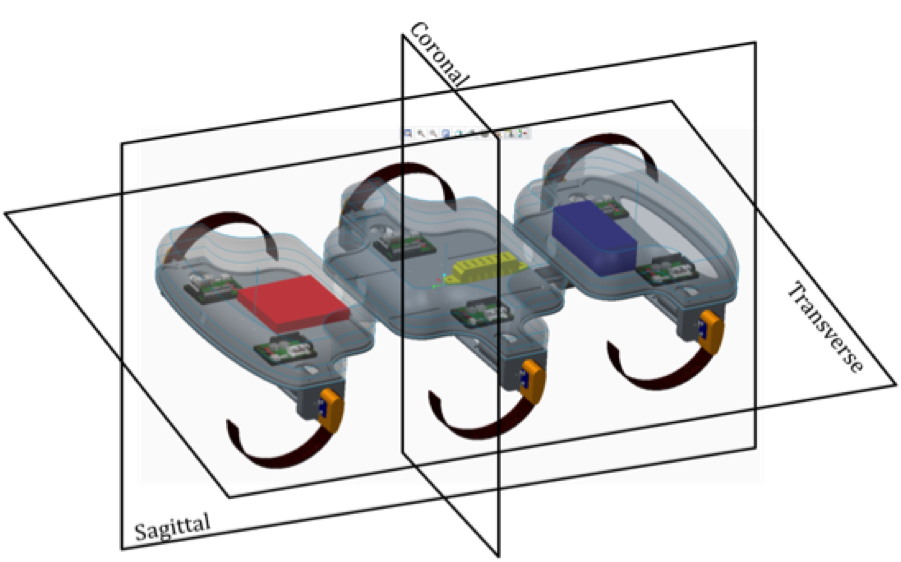
\includegraphics[width=10cm,height=7cm]{bodyplanes.png}
\caption{Isometric view of the segmented body and labeled planes of the body-axis reference frame}
\end{figure}

\subsection{Spinal Joints}

The addition of structural flexibility to the hexapodal design potentially increases stability and efficiency traversing obstacles.  It is also intended to expand the range of terrain that the robot is capable of traversing. The segmented design of three chassis elements connected by two passively actuated joints allows this flexibility to be achieved while retaining rigid platforms for the mounting of required hardware. 

The joint is responsible for the six degrees of freedom between each segment pair. Inspired by biological vertebrae, the three rotational degrees of freedom are emphasized, leaving the three translational ones rigid. Compression and restoration of the semicircular legs already conserve some of the energy used in each step. Rotation in the coronal plane is intended to increase this conservation by allowing the segments to roll several degrees with respect to each other within the period of the tripod gait. The second rotational degree of freedom imitates the arching ability of an animal's spine by pitching the segments. This flexible curvature of the robot's chassis in the sagittal plane allows the third set of legs to be in contact with the ground when the slope beneath the robot varies dramatically along its length.  Such an instance occurs while mounting a stair-like obstacle: the front segment pitches upwards allowing the legs of the middle and rear segments to remain in contact with the flat ground until they too encounter the first step. The final degree of freedom in this body-axis frame of reference is rotation between segments in the transverse plane. This freedom allows the robot to turn aside from obstacles and, by affecting the direction of forward progress, naturally leads to a path of steepest descent. Due to our intent of accurately controlling the direction of the robot's locomotion, yawing motion has been deemed unfavorable and will be rigidly restricted.

These locomotive goals are the purpose the joint must serve and, together with certain other restrictions, define its design.  Four degrees of freedom must be rigidly constrained leaving the roll and pitch motions to be passively actuated such that the ideal degree of flexibility is attained. As this is a research project meant to test the effectiveness of such flexibility, the stiffness of the two allowed motions must be tunable, either continuously or in discreet intervals, and capable of a fully rigid condition for comparison. Weight is a significant limiting factor because increasingly powerful motors, required to compensate for a heavier robot, are increasingly expensive. Designers of the very similar EduBot have also emphasized a positive correlation between weight and difficulty in control. The size of the joint system is restricted due to the necessity of fitting it on the robot's chassis segments while retaining enough surface space for hardware. The problem may be reduced to these requirements: restriction of four degrees of motion and a compact, adjustable method of passive actuation for the remaining two degrees.

\begin{figure}[t]
\begin{minipage}[b]{0.45\linewidth}
\centering
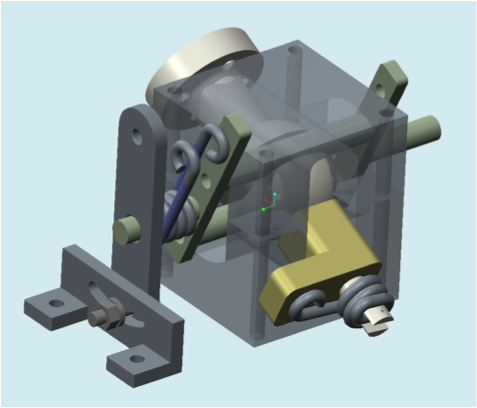
\includegraphics[width=6cm,height=6cm]{joint1.png}
\caption{First joint design: uses torsion springs to passively activate the roll and pitch motions of the ball-axle\\\\}
\label{fig:originaljoint}
\end{minipage}
\hspace{0.5cm}
\begin{minipage}[b]{0.45\linewidth}
\centering
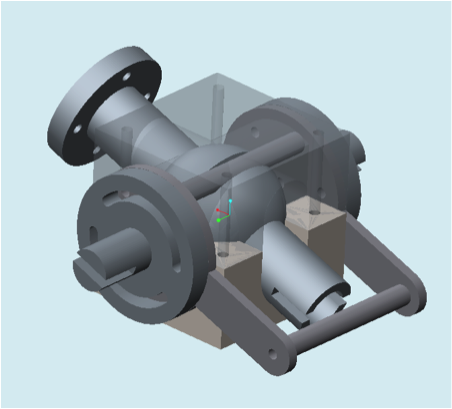
\includegraphics[width=6cm,height=6cm]{joint2.png}
\caption{Second joint design: uses cantilever beams fit through the two open slots to apply restoring torques to these motions. Each had an adjustable equilibrium pitch angle}
\label{fig:secondjoint}
\end{minipage}
\end{figure}

The original design was based around a ball joint with a protruding axle (see Figure \ref{fig:originaljoint}). With the joint's housing mounted to the middle segment and the end of the axle attached to either end segment, the axle's rotations allow the segment pairs to pitch and roll with respect to each other. Furthermore, the two degrees of freedom within the joint can be mechanically and independently controlled: pitch rotation via a fork slotted through the ball, and roll rotation at the back end of the axle. Either of the motions can be made completely rigid or passively actuated by a single torsion spring without affecting the other. The plan was to simply replace the torsion springs to acquire different degrees of stiffness. However, difficulty arose in the selection of torsion springs, because the estimated dynamic loads on the segments required torques of up to 60 lbf-in at the joint. Achieving this torque, after less than 20 degrees of rotation, requires a level of stiffness such that the spring size becomes cumbersome. Larger springs require a scaled up joint and this became a rather dense design, involving relatively large volumes of plastic and metal.

The next variation sought to preserve the ball joint design while replacing the too large torsion springs with more compact and continuously adjustable thin, cantilever beam springs which would have a moment applied around the free end. The desired maximum angles of pitch and roll created stress in the beam such that its length had to be too long to fit on top of the chassis with the rest of the joint system.


\begin{figure}[t]
\begin{minipage}[b]{0.45\linewidth}
\centering
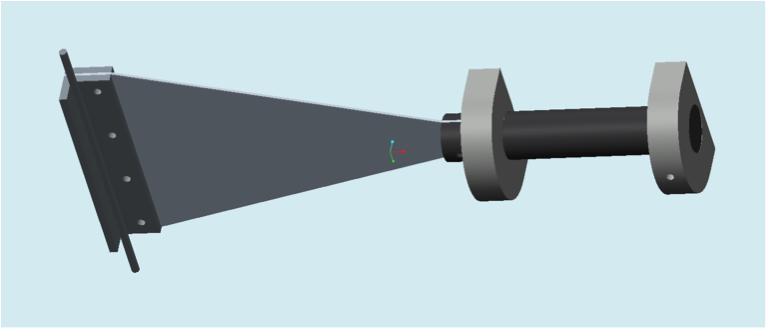
\includegraphics[width=8cm,height=5cm]{joint3.png}
\caption{Third joint design: relied upon a welded pin and a polyurethane torsion rod\\\\\\}
\label{fig:thirdjoint}
\end{minipage}
\hspace{0.5cm}
\begin{minipage}[b]{0.45\linewidth}
\centering
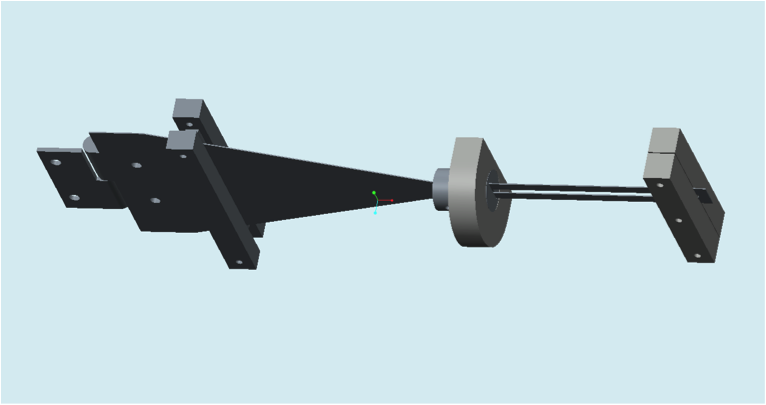
\includegraphics[width=8cm,height=5cm]{joint4.png}
\caption{Current joint design: replaced the pin with a hinge, torsion rod with a narrow extension of the same plate, and includes the translatable fulcrum for adjusting stiffness in pitch}
\label{fig:fourthjoint}
\end{minipage}
\end{figure}

At this point in the design process it was decided that the joint was becoming too complicated and a new track was taken, combining the two previously summarized requirements into a single solution. Rather than create a rigid joint which allows motion in only the two desired degrees of rotation and then add a system of passive actuation to it, the joint itself could be made from a flexible material. The cantilever thin beam spring from the prior version can be increased in length and width to handle the stress, providing pitch flexibility as well as the structural connection between segments. Roll flexibility requires a much narrower extension of the plate which is otherwise too rigid in that mode of torsion (see Figure \ref{fig:thirdjoint}). By relocating the beam spring to the underside of the chassis, space is preserved on top for the hardware.

The bending dynamics of a cantilever beam result in the maximum stress occurring at the clamped end; the stress then decreases linearly to zero at the loaded end. By tapering the width of the beam, the stress can be made constant throughout the spring and a greater deflection and angle of deflection acquired at the load end without raising the maximum stress (see Figure~\ref{fig:jointplots1}). However, this creates a problem with adjusting the stiffness. As the location of the clamp is moved towards the load end in order to stiffen the joint, the maximum stress is occurring at an increasingly small cross section and so increases. In order to prevent stress from increasing with stiffness, the cantilever beam was replaced by an overhanging beam pinned at the base and simply supported from an adjustable fulcrum. By moving the fulcrum towards the load end, the spring can be stiffened while still utilizing the length of the beam behind the fulcrum, unlike with the clamped cantilever. With this pinned, over-hanging beam, the maximum stress occurs at the fulcrum and decreases as the fulcrum moves towards the loaded end (see Figure~\ref{fig:jointplots2}). This serves to counteract the increasing stress caused by the tapered width and shrinking cross sectional area. The over-hanging beam maximizes the ratio of end deflection to stress and allows for an adjustable stiffness without significantly changing the maximum stress.

\begin{figure}[H]
\centering
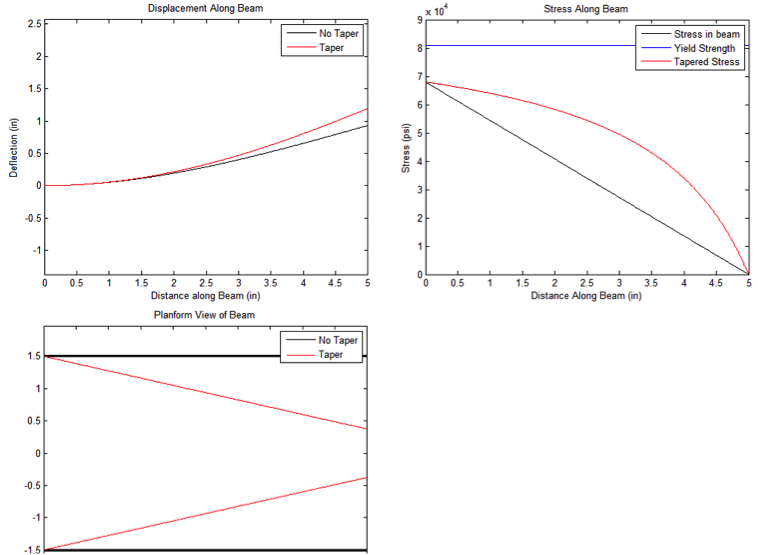
\includegraphics[]{jointgraphs1.png}
\caption{Plots of deflection, stress, and planform shape of the cantilever beam comparing a constant width (black) with tapered (red).}
\label{fig:jointplots1}
\end{figure}

\begin{figure}[H]
\centering
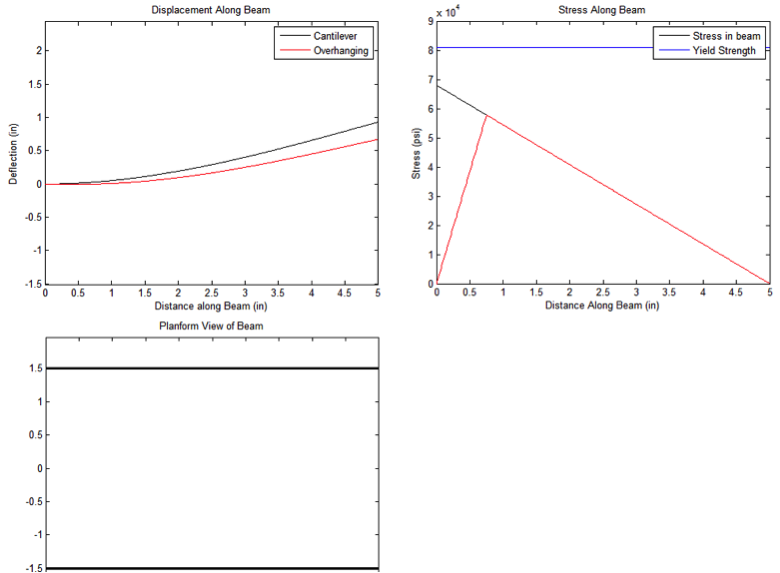
\includegraphics[]{jointgraphs2.png}
\caption{Plots of deflection, stress, and planform shape comparing cantilever (black) to overhanging (red) type beam. The overhanging beam sacrifices some deflection for less stress and adjustable stiffness. The fulcrum of the overhanging beam is located 0.75in from the pinned end in this instance.}
\label{fig:jointplots2}
\end{figure}

\begin{figure}[H]
\centering
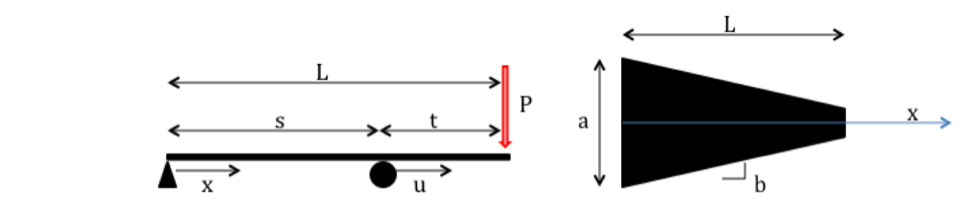
\includegraphics[width=14cm,height=3cm]{jointfbd.png}
\caption{Left: Supports for triangular section of joint. Right: planform view}
\end{figure}

\begin{center}
$\sigma_{max} = \frac{M_{max}c}{I} = \frac{P*t*\frac{h}{2}}{w*\frac{h^3}{12}} = \frac{6P}{h^2}\frac{L-s}{w}$ \\
$w = a(1-bs) = \frac{a}{L}(L-bLs)$ \\
$\sigma_{max} = \frac{6P}{h^2}\frac{L-s}{\frac{a}{L}(L-bLs)} = \frac{6PL}{ah^2}\frac{L-s}{L-bLs}$ \\
As b $\rightarrow \frac{1}{L}$ $\sigma_{max} =  \frac{6PL}{ah^2}$, \bf{constant} 
\end{center}

\vspace{0.5cm}

\begin{center}
deflection at x = $\frac{1}{EI}(\frac{Pt}{6s}x^3 - \frac{Pts}{6}x)$ \\
deflection at u = $\frac{1}{EI}(\frac{Pt}{2}u^2 - \frac{P}{6}u^3 + \frac{Pts}{3}u)$
\end{center}

\subsection{Electronic System}

In order to provide actuation in a stable and precise manner we chose a pre-assembled EPOS PID control system provided by Maxon Motors\footnote{Maxon Motors, \url{http://www.maxonmotorusa.com/}} combined with a BeagleBoard-XM single-board computer\footnote{Beagleboard XM, \url{http://beagleboard.org/hardware-xm}}. On a modular scale, the components are arranged in the manner shown in Figure \ref{fig:closedloop} to implement closed loop control.

\begin{figure}[H]
\centering
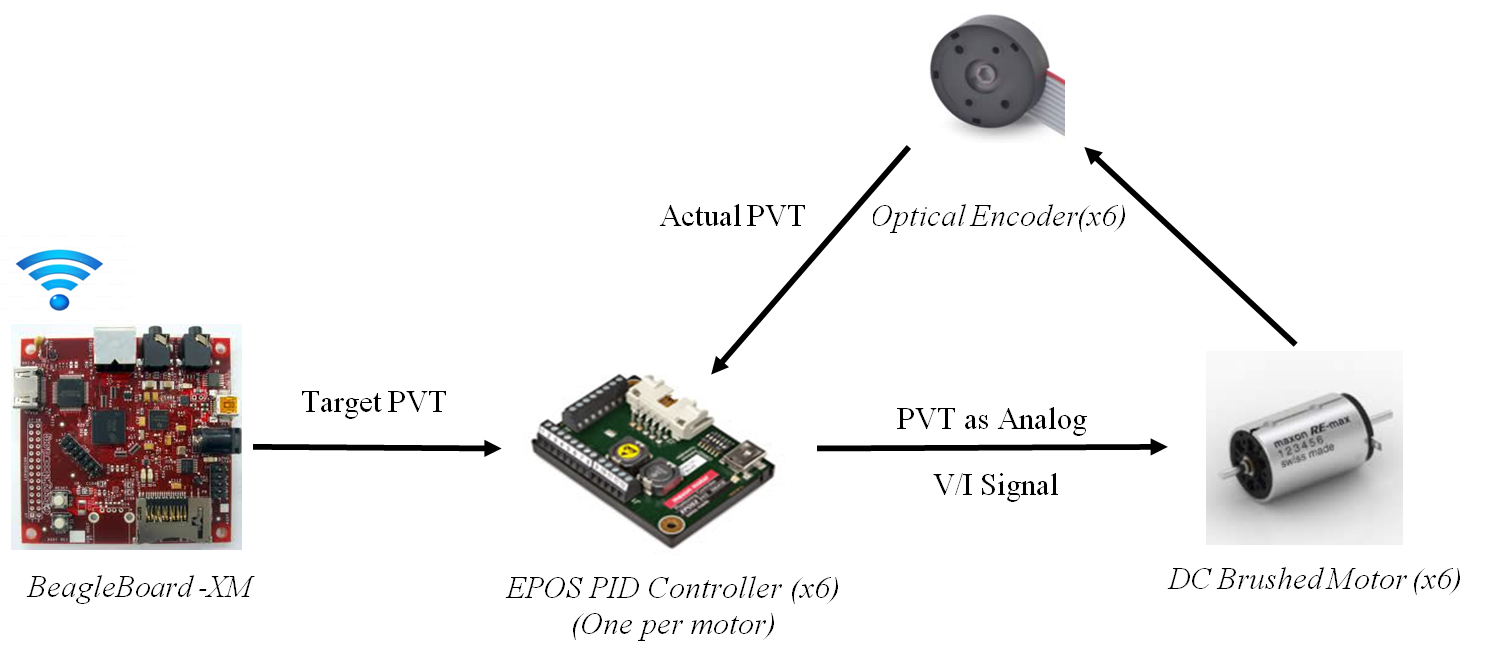
\includegraphics[width=14cm,height=6.5cm]{macro_ControlLoop_PAYNE.png}
\caption{Control Loop}
\label{fig:closedloop}
\end{figure}

On this scale, the user accesses the BeagleBoard-XM via WiFi to initiate a particular high-level locomotion routine. This routine ranges from simple in nature – such as “move forward a half meter” to more complex functions such as “move towards most prominent lightsource”. The BeagleBoard-XM, running Python/C++ scripts on Linux, then calls the appropriate EPOS microcontroller API methods in order to execute the associated Position, Velocity, Time (PVT) trajectory as generated with the control algorithms described in the simulation section.

In order to efficiently communicate between the BeagleBoard-XM and each of the EPOS controller units, a CAN network is utilized. We assign each controller in the network a particular node ID by aligning binary DIP switches on the controller. All the nodes are then linked together via a serial CAN COMM consisting of a CAN High and CAN Low line, with all nodes commonly grounded. We wound the three lines together in order to provide equal capacitance throughout the network to minimize noise interference. Finally, a master node links the CAN network via USB to the controlling BeagleBoard-XM. When a packet is sent using the CAN network standard, its contents are read by only the node that corresponds to the node ID found in the packet’s header.

It should be noted that at this time we are only using two nodes that are connected to our laptop via the USB protocol. We are currently using the EPOS Controller PC GUI, rather than the Linux EPOS Controller API, to control the two motors on our test rig. The GUI provides an intuitive interface to use as we learn how to control the motors at the expense of having limited functionality especially when attempting to synchronize node behavior.  Once we have finished this testing phase, we will develop scripts that call the EPOS Controller API in order to control all six nodes in a precise and synchronous manner.

\begin{figure}[H]
\centering
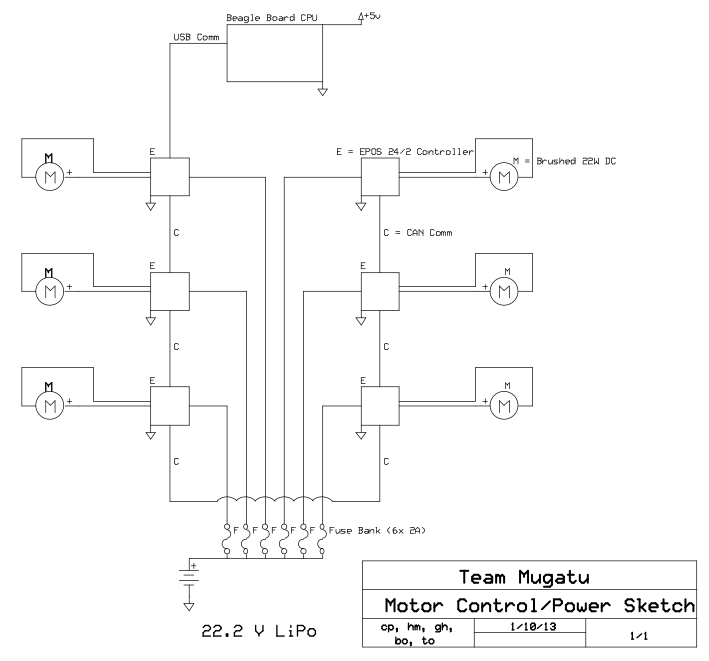
\includegraphics[width=15cm,height=14cm]{motorcontrolsketch.png}
\caption{Circuit diagram of our design, demonstrating the communications network and power system}
\label{fig:motorcircuit}
\end{figure}

\section{Test Rig}

\begin{figure}[t]
\centering
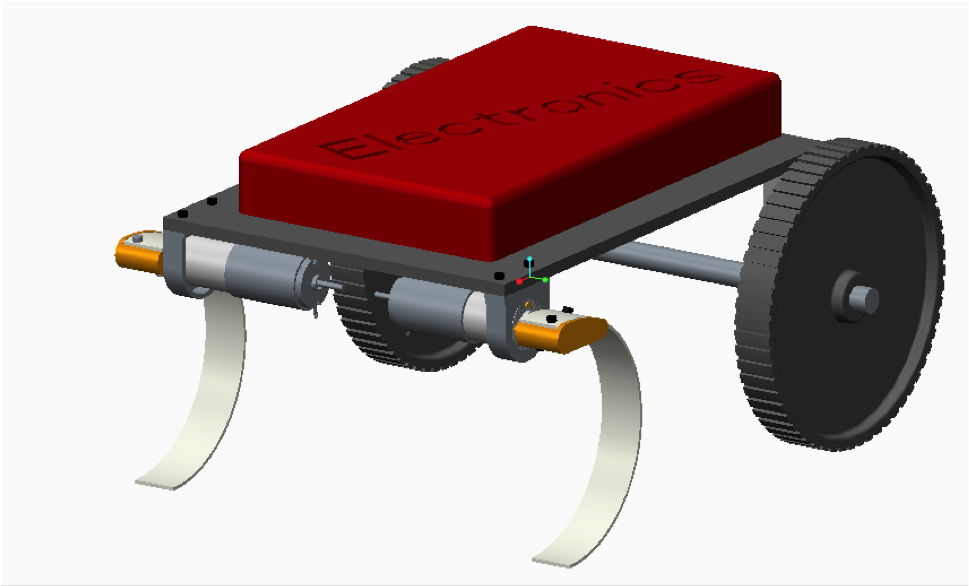
\includegraphics[width=8cm,height=6cm]{cad_test_cart.png}
\caption{CAD model of the test cart}
\label{fig:testcart}
\end{figure}

The test cart (Figure \ref{fig:testcart}) was constructed to demonstrate the operation of our mechatronic systems. It has two legs instead of our final six to simplify construction, wiring, and programming. The back of the test cart is supported by two wheels, giving the rig additional stability and allowing it to stand on one of the two front legs.

Because the test cart is a simplified version of the final robot, the specifications and methods of construction are as close to those of our final robot as possible. The platform of the cart is made of a sheet of PVC plastic, which was chosen because of its low cost and ease of machining. The front legs are bent into 7" diameter semicircles, which is the preliminary size of the legs that will be used on the final robot. The legs themselves are made of one inch wide strips of 0.072" thickness spring steel, which was chosen for the six legged robot based on finite element analysis conducted in Creo (see Figure \ref{fig:legstress}). The two-piece joint that affixes the steel leg to the motor was machined out of aluminum to the specifications of the final robot. The aluminum motor mounts, which were machined using a mill for the test cart, will be machined using CNC for the final robot.

Currently, the test cart is capable of successful basic locomotion. We are able to generate trajectories on a laptop and send commands to the network of motor controllers, which then power the legs with various gaits. The next step is to write software for our onboard CPU such that the cart does not need to be tethered to a laptop. Overall, power and torque observations made about the test cart match up well both with our initial calculations and results from simulation studies. Progress on the project has suffered no major setbacks, and we proceed on schedule toward the construction of our main prototype.

\section{Acknowledgements}

This work is funded by the Princeton University School of Engineering and Applied Science, the Department of Mechanical and Aerospace Engineering, and the Department of Electrical Engineering. 

The authors would like to thank Professors Daniel Nosenchuck, Phillip Holmes, and Andrew Houck for acting as advisers, and Dr. Haldun Komsuoglu for providing invaluable support.

\end{document}